\newpage
\section{Continuous Interior Penalty Method}%
\label{sec:continious_interior_penalty_method}


\subsection{Introduction}%
\label{sub:introduction}

To solve \eqref{eq:bi_problem} numerically do we want to introduce the continuous interior penalty method (CIP), which is a discontinuous Galerkin
method (DG) using $C^{0}$ finite elements. There is several reasons why we want to apply nonconformal $C^{0}$ instead of the often used conformal $C^{1}$ finite elements for fourth order problems.

However, it is known that $ H^{2}$ conforming methods requires global $C^{1}$ continuity \cite{ye19}, and creates difficulties creating elements which conserves this property. Some examples is the Argyris element, but it has been shown to be fairly
complicated because you have to construct 21 degrees of freedom for triangle elements \cite{ nair21, brenner07math}. However, some sources tend to say that this method outperforms traditional $C^{0}$ methods \cite{kirby18}, but it still seems to be rarely applied.
Nevertheless, it has also been shown DG methods that is conform and has no penalty terms that does converge \cite{ye19}. Hence, makes the method simpler since it does not involve tuning of penalty parameters, thus might be promising. None of these conform methods mentioned has shown to retain the same properties in 3D.

For the CIP case is $C^0$ finite elements much simpler than obtaining $C^{1}$ finite elements. Also, compared to other similar methods such as the mixed finite element method, CIP does in fact preserve the symmetric positive definiteness, which means
the stability analysis is more straight forward. Finally and most importantly, according to \cite{brenner2012quadratic} can naive use mixed methods of splitting the boundary conditions of
the problem \eqref{eq:bi_problem} produce wrong solutions if $\Omega $ is non convex.

\subsection{Computational Domains}%
\label{sub:computational_domain}

Let $\mathcal{T}  = \left\{ T \right\} $ be a triangulation of $\Omega \subset   \mathbb{R} ^2 $ consisting of triangles $T$. We may also define the set of all facets $\mathcal{F}_{h}$, where every facet is denoted by $F \in \mathcal{F} _{h}$. However, we will distinguish between the
set of external facets $\mathcal{F}^{ext} _{h}$, which is all facets along $\partial \Omega $, and the interior facets $\mathcal{F} ^{int}_{h}$. Let the facets be denotes as $F \in \mathcal{F } _{h}$, then the normal vector $n$ is across the facets from
$T^{+}$ to $T^{-}$, illustrated in figure \ref{fig:normal}.

\begin{figure}[!h]
\centering
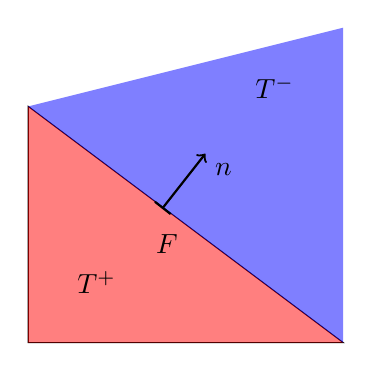
\begin{tikzpicture}[scale=1]
\coordinate (A) at (0,0);
\coordinate (C) at (0,3);
\coordinate (B) at (4,0);
\coordinate (D) at (4,4);
\coordinate (Tm) at (3.5,3.5);
\coordinate (Tp) at (0.5, 0.5);
\coordinate (e) at (1.5, 1.5);
\coordinate (start) at (1.7, 1.7);
\coordinate (end) at (2.25, 2.4);

\draw (A) -- (B) -- (C) -- cycle;
\fill[red, opacity=0.5] (A) -- (B) -- (C);
\fill[blue, opacity=0.5] (B) -- (C) -- (D);
\node[below left] at (Tm) {$T^{-} $ };
\node[above right] at (Tp) {$T^{+}$ };
\node[below right] at (e) {$F$ };

\draw [|->, thick] (start) -- (end);
% \node[above right] at (A) {A };
% \node[below right] at (B) {B};
% \node[above right] at (C) {C };
% \node[below right] at (D) {D};
\node[below right] at (end) {$n$};
\end{tikzpicture}
\caption{Facet $F \in \mathcal{F}_h $ shared by the triangles $T^{+}, T^{-} \in \mathcal{T}_{h} $ and the normal unit vector $n$.  }
    \label{fig:normal}
\end{figure}

A parameter which is useful is the maximum diameter $h$ of the set of triangles $\left\{ T \right\} $, which we to be defined such that,

\begin{equation}
\begin{split}
    h _{T} & = diam\left( T \right)   = \max_{x_1, x_{2} \in T} dist(x_{1}, x_{2}),  \\
    h_{min} & = \min_{T \in \mathcal{T} } h_{T}, \\
    h_{max} &= \max_{T \in \mathcal{T} }  h_{T} := h,
\end{split}
.\end{equation}




where the $diam( T )$ is the largest facet for a triangle $T$. We will also assume mesh conform i.e., if $T_{1} \neq T_{2 }$  and $T \cap T_{2} \neq \emptyset  $ , then they share either a vertex or a facet.

Let the chunkiness parameter $c_{T} := h_{T}/r_{T}$, where $r_{T}$  is the largest ball that be inscribed inside the element $T$. We can then assume that the mesh is shape regular, i.e., that $c_{T}\le  c$ independent of $T$  and $h$. We may also assuming that
the mesh is quasi-uniform only if it holds that the mesh is shape regular and $h_{max} \le  c h_{min}$.




\subsection{Constructing Continuous Interior Penalty Method}%
\label{sub:constructing_continious_interior_penalty_method}

 Let us assume that $u,v \in
H^{4}\left( T  \right) $. Using that the weak form identity \eqref{eq:weak_form_identity} also holds for a triangle $T$ can we write
\begin{equation}
\label{eq:bi_basic_dg}
\left( \Delta  ^{2} u,v \right) _{T} =  \left( D^2u,D^2v \right) _{T } - \left(\partial _{nt} u, \partial _{t}v
\right)_{\partial T} - \left(\partial _{nn} u, \partial _{n}v \right)_{\partial T} + \left(\partial _{n} \Delta  u,v
\right)_{\partial T}
.\end{equation}
For global continuity, let  $v \in V =  \left\{ v \in H^{1}\left( \Omega  \right): v_{T} \in  H^{4}\left( T \right), \ \forall T \in
\mathcal{T}_{h}    \right\} $ and $u \in  H^{4}\left( \Omega  \right) $ such that,

\begin{equation}
\label{eq:bi_basic_dg2}
\left( \Delta  ^{2} u,v \right) _{\Omega } = \sum_{T \in  \mathcal{T} _{h}}^{}  \left( D^2u,D^2v \right) _{T } - \left(\partial _{nt} u, \partial _{t}v
\right)_{\partial T} - \left(\partial _{nn} u, \partial _{n}v \right)_{\partial T} + \left(\partial _{n} \Delta  u,v
\right)_{\partial T}.
\end{equation}
However, this expression can be written to distinguish integrating over triangles $\mathcal{T} _{h}$ , integrating over exterior facets $\mathcal{F} _{h}^{ext}$ and then integrate interior facets $\mathcal{F} _{h}^{int}$.

\begin{equation}
\label{eq:bi_basic_dg_full_1}
\begin{split}
\left( \Delta  ^{2} u, v \right) _{\Omega } =& \sum_{T \in  \mathcal{T} _{h}}^{} \left( D^2u, D^2v \right)_{T}    \\
& + \sum_{F \in \mathcal{F}_{h}^{ext}}  \left(\partial _{n} \Delta u, v  \right) _{F} - \left(\partial _{nt} u, \partial _{t} v \right) _{F}-
\left( \partial _{nn} u, \partial _{n} v \right)_{F}  \\
& + \sum_{F \in \mathcal{F}_{h}  ^{int}}^{} \left(\partial _{nn} u , \jump{ \partial _{n} v }
\right)_{F} \\
& = \sum_{T \in  \mathcal{T} _{h}}^{} \left( D^2u, D^2v \right)_{T} + \sum_{F \in
\mathcal{F} ^{ext}_{h}}^{} \left(g, v  \right) _{F}
  + \sum_{F \in \mathcal{F}_{h}  ^{int}}^{} \left( \partial _{nn} u , \jump{ \partial_{n} v } \right)_{F}
\end{split}
\end{equation}
Keep in mind that any jump over a interior facet $F \subset \mathcal{F} _{h}^{int}   $, visualized in figure \ref{fig:normal}, is defined as $\jump{ a } =    a^{+} - a^{-} $
and likewise for the mean, $\mean{ a  } = \frac{1}{2}(   a^{+}
+ a^{-})$.    The equivalence of \eqref{eq:bi_basic_dg2} and \eqref{eq:bi_basic_dg_full_1} comes from the following argumentation.

\begin{equation*}
    \begin{split}
 \left( \Delta  ^{2} u,v \right) _{\Omega } & =\sum_{T\in \mathcal{T} _{h}}^{} \left( D^2u,D^2v \right) _{T } - \left(\partial _{nt} u, \partial _{t}v
\right)_{\partial T} - \left(\partial _{nn} u, \partial _{n}v \right)_{\partial T} + \left(\partial _{n} \Delta  u,v
\right)_{\partial T} \\
&= \sum_{T\in \mathcal{T} _{h}}^{} \left( D^2u,D^2v \right) _{T } \\
&  \quad + \sum_{F \in \mathcal{F}_{h}^{ext} }^{} \underbrace{\left( \partial _{n} \Delta  u, v  \right)_{F}}_{= \left( g,v \right)_{F} }  -  \left(
\partial _{nt} u, \partial _{t} v \right) _{F}  - \underbrace{\left( \partial _{nn} u, \partial _{n} v \right)_{F}}_{ = 0}    \\
& \quad  + \sum_{F \in \mathcal{F} _{h}^{int}}^{} \underbrace{\left( \left(\partial _{n^{+}} \Delta  u^{+}
        ,v^{+}\right)_{F}
+ \left(\partial _{n^{-}} \Delta  u^{+} ,v^{-}\right)_{F}  \right)}_{(I)} \\
 & \quad \quad \quad  \quad +
\underbrace{\left( \left(\partial _{n^{+}t} u^{+}, \partial_{t} v^{+} \right)_{F} +  \left(\partial _{n^{-}t} u^{-},
        \partial_{t} v^{-}
\right)_{F}  \right) }_{(II)} \\
 & \quad \quad \quad  \quad  +
\underbrace{\left( \left(\partial _{n^{+}n^{+}} u^{+}, v^{+} \right) _{F} + \left(\partial _{n^{-}n^{-}} u^{-}, v^{-}
\right) _{F} \right) }_{(III)}
    \end{split}
.\end{equation*}

Where integration over all interior facets $ \forall F \in \mathcal{F}_{h}^{int}$ is computed in this way.
\begin{equation*}
    \begin{split}
        (I) &  =    \left(\partial _{n^{+}} \Delta  u^{+} ,v^{+}\right)_{F} +
        \left(\partial _{n^{-}} \Delta  u^{-} ,v^{-}\right)_{F}  \\
        & =   \int_{F}^{}
        \jump{ \partial _{n} \Delta  u \cdot v } =
         \int_{F}^{}
         \mean{ \partial _{n} \Delta  u } \underbrace{\jump{ v }}_{= 0}    + \underbrace{\jump{ \partial _{n} \Delta  u
         }}_{= 0}    \mean{ v } = 0 \\
        (II) &  =     \left(\partial _{n^{+}t} u^{+}, \partial_{t} v^{+}
        \right)_{F} +  \left(\partial _{n^{-}t} u^{-}, \partial_{t} v^{-}
\right)_{F}   \\
&  =   \int_{F}^{}
        \jump{ \partial _{nt} u \cdot  \partial_{t} v } =
         \int_{F}^{}
         \mean{ \partial _{nt} u    } \underbrace{\jump{ \partial_{t} v }  }_{= 0}    + \underbrace{\jump{ \partial
                 _{nt}  u
         }}_{= 0}    \mean{ \partial _{t}v }  = 0\\
        (III) &  =     \left(\partial _{n^{+}n^{+}} u^{+}, \partial_{n^{+}} v^{+} \right)_{F} +  \left(\partial _{n^{-}n^{-}} u^{-}, \partial_{n^{-}} v^{-} \right)_{F}    =    \int_{F}^{} \jump{ \partial _{nn} u \cdot  \partial_{n} v }  \\
        & = \int_{F}^{}
        \mean{ \partial _{nn} u    } \underbrace{\jump{ \partial_{n} v }  }_{\neq 0}    + \underbrace{\jump{ \partial
                 _{nn}  u
         }}_{= 0}    \mean{ \partial _{n}v }   =  \left( \partial _{nn} u, \jump{ \partial_{n} v } \right)_{F}   \end{split}
.\end{equation*}
Observe that the cancellations in the term $(I)$ appears of the continuity of $v\in V $ and $u\in H^{4}\left( \Omega  \right) $ which makes the jumps zero. For the second term $(II)$ does the terms become zero cancelled because the tangential
derivative at the facet has no jump. However, The third term $(III)$  is fairly interesting since the discontinuity in
normal vector for $v \in V$ is a jump, while the second term is still continuous. It can also be raised that $\mean{
\partial _{nn} u } = \partial _{nn} u  $ holds by the continuity of $H^{4}\left( \Omega  \right) $. Hence,
\eqref{eq:bi_basic_dg2} and \eqref{eq:bi_basic_dg_full_1} is equivalent.

\subsection{Formulation of the Continious Interior Penalty Method}%
\label{sub:formulation_of_continious_interior_penalty_method}


We can finally start defining the fully discrete formulation. Let the basis be a $\mathcal{P}_{2} $ Lagrange finite element space so,
\[
V_{h} = \left\{ v \in C^{0}\left( \Omega  \right): v_{T} = v | _{T} \in \mathcal{P} _{2}\left( T \right), \forall T \in
\mathcal{T}_{h}    \right\}
\]
and
\[
V_{h}^{*} = \begin{cases}
    V_{h} & \text{ if } \alpha  > 0 \\
    \left\{ v \in V_{h}: \int_{\Omega }^{} v dx   = 0   \right\} &  \text{ if } \alpha   = 0
\end{cases}
\]
Now, if we choose $u \in V_{h}$, then we must take account that the jump is discrete.
 Finally, the CIP formulation can be stated as follows.
The discretized numerical problem is to solve $w_{h} \in V_{h}^{*}$ such that
\begin{equation}
\label{eq:CP_A_F}
\mathcal{A}\left( w_{h}, v_{h} \right)   = F\left( v_{h} \right), \quad \forall v_{h} \in V_{h}^{*}  .
\end{equation}
where
\begin{equation}
\label{eq:CP_A_h_1}
\begin{split}
\mathcal{A} \left( w_{h}, v_{h} \right)   =&
  \quad  \left( \alpha  w_{h}, v_{h} \right) _{\Omega }\\
&  + \sum_{T \in \mathcal{T} _{h}}^{} \left( D^2 w_{h}, D^2v_{h} \right) _{T} \\
 & +
  \sum_{F \in \mathcal{F}_{h}^{int} }^{}
  \left( \mean{  \partial _{n n} w_{h} }, \jump{ \partial _{n }v_{h}} \right)_{F}  +
 \left( \mean{ \partial _{n n} v_{h} }, \jump{ \partial _{n}w }      \right)_{F} \\
& \quad \quad \quad \quad  + \frac{\gamma}{h}  \left( \jump{ \partial _{n} w_{h}}, \jump{ \partial _{n} v_{h}   }   \right)_{F}
\end{split}
\end{equation}
and
\begin{equation}
\label{eq:CP_F_h}
F\left( v_{h} \right)  = \left( f, v_{h} \right) _{\Omega } +  \sum_ {F \in \mathcal{F}_{h} ^{ext}}^{} - \left(g, v_{h}  \right) _{F}.
\end{equation}
Notice that the regulation term determined by respectively a global tuning parameter $\gamma >0 $. Another key component to the formulation
in \eqref{eq:CP_A_h_1} after introduction of $ w_{h}, v_{h} \in V^{*}_{h}$  is that we expanded $\left( \partial _{nn}w, \jump{ \partial _{n} v }  \right)_{F} \to \left( \mean{ \partial _{nn}w_{h} }  , \jump{ \partial _{n} v_{h} }  \right)_{F} $ since we can longer not guarantee a
continuous jump. For symmetric purposes we also added $ \left( \mean{ \partial _{nn} v_{h}}  , \jump{ \partial _{n} w_{h} }  \right)_{F} $. For convenience will we introduce the compact notation of \eqref{eq:CP_A_h_1},

\begin{equation}
\label{eq:CP_A_h}
\begin{split}
\mathcal{A} \left( w_{h}, v_{h} \right)   =&
  \quad  \left( \alpha  w_{h}, v_{h} \right) _{\Omega }\\
&  +  \left( D^2 w_{h}, D^2v_{h} \right) _{\mathcal{T} _{h}} \\
 & +
  \left( \mean{  \partial _{n n} w_{h} }, \jump{ \partial _{n }v_{h}} \right)_{\mathcal{F}_{h}}  +
 \left( \mean{ \partial _{n n} v_{h} }, \jump{ \partial _{n}w }      \right)_{\mathcal{F}_{h}}
 \\
 & + \frac{\gamma }{h}  \left( \jump{ \partial _{n} w_{h}}, \jump{ \partial _{n} v_{h}   }   \right)_{\mathcal{F}_{h}} \\
\end{split}
.
\end{equation}

\subsection{ Stability Results}%
\label{sub:error_and_stability_analysis_of_c0ip}

To guarantee convergence and stability we may want to check coercivity and boundedness of the method.

First of all, let us now establish some important inequalities.
\[
\begin{split}
    \textbf{Cauchy-Schwarz inequality: } & \| ab \|_{  }^{  }  \le \| a \|_{  }^{  } \| b \|_{  }^{  }   \\
    \textbf{Inverse inequality: } & \frac{1}{h}\| \partial _{nn}  v_{h} \|_{\mathcal{F}_{h}   }^{2  }  \le C_{j} \| D ^2 v_{h} \|_{ \mathcal{T} _{h} }^{ 2 }   \\
    \textbf{Youngs epsilon inequality: } & 2ab =   2\sqrt{\varepsilon }a\cdot    \frac{b}{\sqrt{\varepsilon } } \le \varepsilon a^2+ b^2 \frac{1}{\varepsilon }
\end{split}
\]

Let the energy norm be on the form,
\begin{equation}
\label{eq:A_energy_norm}
    \begin{split}
\| v_{h} \|_{ h }^{2  } & = \| v_{h} \|_{ a_{h} }^{ 2 } =  \| v_{h} \|_{ \Omega  }^{2  }  +  \| D ^2 v_{h} \|_{ \mathcal{T} _{h}  }^{ 2 }  + \|  h^{-\frac{1}{2}} \jump{ \partial _{n} v_{h}    }\|_{  \mathcal{F} _{h} }^{2  }, \\
\| v \|_{ h }^{ 2 }  &= \| v \|_{ a_{h},* }^{ 2 } = \| v \|_{ a_{h} }^{ 2 }  + \| h^{\frac{1}{2}} \left\{ \partial _{nn } v\right\}  \|_{ \mathcal{F}_{h}   }^{  2}, \quad  v\in V \oplus V_{h}.
    \end{split}
\end{equation}
The method is said to be coercive if $\mathcal{A} _{h}\left( v_{h}, v_{h} \right) \ge  C \| v_{h} \|_{ a_{h} }^{  } $. Similarly, it is bounded if $ \mathcal{A} _{h} \left( v_{h}, u_{h} \right) \le  C \| u_{h} \|_{  a_{h}}^{ 2 }  \| v_{h} \|_{ a_{h}
}^{ 2 } $ and then, according to Lax Milgram the problem is said to be well posed.

\subsubsection{Coercivity}%
\label{ssub:coercitivity}


Suppose we have the CIP problem described in \eqref{eq:CP_A_F}. Then is the coercivity be computed such that,
\[
    \begin{split}
\mathcal{A} \left( v_{h}, v_{h} \right)  =& \quad  \alpha \|  v_{h}  v_{h} \|_{ \Omega  }^{  } +  \| D^2v_{h} \|_{ \mathcal{T} _{h} }^{2  }   \\
& \quad + 2 \left(  \mean{ \partial _{nn} v_{h} }    ,  \jump{ \partial _{n}v_{h} }     \right) _{\mathcal{F} _{h}} +  \frac{\gamma}{h} \|  \jump{ \partial _{n} v_{h} }
  \|_{ \mathcal{F} _{h} }^{ 2 } \\
\quad \textit{Cauchy-Schwarz inequality} \quad
 \ge& \quad  \alpha \| v_{h}  \|_{\Omega   }^{  } \| v_{h} \|_{\Omega   }^{  } +   \| D ^2 v_{h} \|_{ \mathcal{T} _{h} }^{2  } \\
& \quad -2 \| h^{\frac{1}{2}} \mean{ \partial _{nn}v_{h} }    \|_{  \mathcal{F} _{h}}^{  } \| h^{-\frac{1}{2}} \jump{ \partial _{n}v_{h} }    \|_{  \mathcal{F} _{h}}^{  } + \gamma \| h^{-\frac{1}{2}}  \jump{ \partial _{n}v_{h} }   \|_{ \mathcal{F} _{h}  }^{ 2 } \\
\quad \textit{Inverse inequality} \quad
   \ge & \quad  \alpha \| v_{h}  \|_{\Omega   }^{  } \| v_{h} \|_{\Omega   }^{  } + \| D ^2 v_{h}  \|_{ \mathcal{T} _{h}  }^{ 2  }  \\
 &  \quad - 2 C^{\frac{1}{2}}_{j} \|   D ^2 v_{h}    \|_{ \mathcal{T} _{h}  }^{  } \| h^{-\frac{1}{2}} \jump{ \partial _{n} v_{h} }   \|_{ \mathcal{F} _{h} }^{  }  + \gamma \| h^{ -\frac{1}{2}} \jump{
 \partial _{n } v_{h}}   \|_{ \mathcal{F}_{h}}^{2}  \\
\quad \textit{ Youngs epsilon inequality} \quad
    \ge  &  \quad  \alpha \| v_{h}  \|_{\Omega   }^{  } \| v_{h} \|_{\Omega   }^{  } +  \| D ^2 v_{h} \|_{ \mathcal{T}_{h}  }^{2  } - \varepsilon C_{j} \| D ^2 v_{h} \|_{ \mathcal{T} _{h} }^{2  } \\
  & \quad  - \frac{1}{\varepsilon } \| h^{\frac{1}{2}} \jump{ \partial _{n} v_{h} }   \|_{ \mathcal{F} _{h} }^{2  }  + \gamma \|
  h^{-\frac{1}{2}} \jump{ \partial _{n} v_{h}}   \|_{ \mathcal{F} _{h} }^{2  }  \\
   =&  \quad  \alpha \| v_{h}  \|_{\Omega   }^{  } \| v_{h} \|_{\Omega   }^{  } +\left( 1 - \varepsilon C_{j} \right) \| D ^2 v_{h} \|_{\mathcal{T} _{h}  }^{ 2 }  \\
  & \quad + \left( \gamma  - \frac{1}{\varepsilon } \right) \| h^{-\frac{1}{2}} \jump{ \partial _{n} v_{h} }   \|_{ \mathcal{T} _{h} }^{ 2 } \\
  (\varepsilon  = \frac{1}{2 C_{j} })  \implies  \quad \quad =& \quad  \alpha \| v_{h}  \|_{\Omega   }^{  } \| v_{h} \|_{\Omega   }^{  } +\frac{1}{2} \| D ^2 v_{h} \|_{ \mathcal{T} _{h} }^{ 2 }  + \underbrace{\left( \gamma -2 C_{j} \right)}_{ \ge  \frac{1}{2}}  \| h^{\frac{1}{2}} \jump{ \partial _{n} v_{h} }   \|_{
  \mathcal{F} _{h} }^{2  } \\
   \ge & \quad  C \| v_{h} \|_{ a_{h} }^{  2}
    \end{split}
\]
This holds if $C=\min\left\{  \alpha , 1 /2\right\}$.
Observe that for the first inequality is the standard \textbf{Cauchy-Schwarz inequality} such that $$\left( \mean{ \partial_{nn} v_{h} }  , \jump{ \partial _{n} v_{h} }   \right) _{\mathcal{F} _{h}} \ge - \| h^{-\frac{1}{2}} \mean{ \partial _{nn}
v_{h} }    \|_{\mathcal{F}_{h}   }^{  } \| \mean{ \partial _{n}v_{h} }   \|_{ \mathcal{F}_{h}   }^{  } .  $$ On the second inequality the \textbf{Inverse inequality} was applied,
\[
- \| h^{\frac{1}{2}} \mean{ \partial _{nn}v }   \|_{ \mathcal{F} _{h}  }^{  }\ge - C_{j}^{\frac{1}{2}} \| D ^2 v_{h} \|_{ \mathcal{T} _{h} }^{  }
\]
The next step is then to use the \textbf{Youngs epsilon inequality} to separate the facets and triangulation norms, \[
 - 2 C^{\frac{1}{2}}_{j} \|  D ^2 v_{h}    \|_{ \mathcal{T} _{h}  }^{  } \| h^{\frac{1}{2}} \jump{ \partial _{n} v_{h} }   \|_{ \mathcal{F} _{h} }^{  } \ge- \varepsilon C_{j} \| D ^2 v_{h} \|_{ \mathcal{T} _{h} }^{2  } -
 \frac{1}{\varepsilon } \| h^{\frac{1}{2}} \jump{ \partial _{n} v_{h} }   \|_{ \mathcal{F} _{h} }^{2  }
.\]
The last step was to choose a $\varepsilon $ and $\gamma $ as some positive constant so that the second term is restricted to be multiplied with something bigger than $\frac{1}{2}$. Thus, the term fulfils coercivity of the \eqref{eq:A_energy_norm}.
Hence, the CIP method is coercive.

\subsubsection{Boundedness}%
\label{ssub:bounded}
We want the CIP method to be bounded.


\begin{equation*}
    \begin{split}
\mathcal{A} \left( w_{h}, v_{h} \right)   =& \quad \left( \alpha w_{h}, v_{h} \right) _{\Omega } +
    \left( D ^2 w_{h}, D ^2v_{h} \right) _{\mathcal{T} _{h}}
   \\
    &\quad  +
  \left( \mean{  \partial _{n n} w_{h} }, \jump{ \partial _{n }v_{h}} \right)_{\mathcal{F}_{h}}  +
 \left( \mean{ \partial _{n n} v_{h} }, \jump{ \partial _{n}w }      \right)_{\mathcal{F}_{h}} \\
 & \quad + \frac{\gamma }{h}  \left( \jump{ \partial _{n} w_{h}}, \jump{ \partial _{n} v_{h}   }   \right)_{\mathcal{F}_{h}} \\
\quad \textit{Cauchy-Schwarz inequality }\quad  \le& \quad  \alpha  \|  w_{h} \|_{\Omega   }^{  } \| v_{h} \|_{ \Omega  }^{  }     +
\| D ^2w_{h} \|_{\mathcal{T} _{h}   }^{  }  \| D ^2v_{h} \|_{\mathcal{T} _{h}   }^{  } \\
& \quad  + \| h^{\frac{1}{2}}\mean{ \partial _{nn} w_{h} } \|_{ \mathcal{F}_{h}  }^{  } \| h^{-\frac{1}{2}}\jump{ \partial _{n} v_{h} } \|_{ \mathcal{F}_{h}  }^{  }    \\
& \quad  + \| h^{\frac{1}{2}}\mean{ \partial _{nn} v_{h} }
\|_{ \mathcal{F}_{h}  }^{  } \| h^{-\frac{1}{2}}\jump{ \partial _{n} w_{h} } \|_{ \mathcal{F}_{h}  }^{  }  \\
& \quad + \gamma \| h^{-1} \jump{ \partial _{n} v_{h}}   \|_{ \mathcal{F} _{h} }^{  }   \|  \jump{ \partial _{n} w_{h}}   \|_{ \mathcal{F} _{h} }^{  } \\
\quad \textit{Inverse inequality }\quad  \le & \quad   \alpha  \|  w_{h} \|_{\Omega   }^{  } \| v_{h} \|_{ \Omega  }^{  }  +
\| D ^2w_{h} \|_{\mathcal{T} _{h}   }^{  }  \| D ^2v_{h} \|_{\mathcal{T} _{h}   }^{  } \\
& \quad + C_{j}^{\frac{1}{2}} \| D ^2 w_{h} \|_{\mathcal{T} _{h}  }^{  }  \| h^{-\frac{1}{2}}\jump{ \partial _{n} v_{h} } \|_{ \mathcal{F}_{h}  }^{  }
 \\
& \quad +  C_{j}^{\frac{1}{2}} \| D ^2 w_{h} \|_{\mathcal{T} _{h}  }^{  }
 \| h^{-\frac{1}{2}}\jump{ \partial _{n} w_{h} } \|_{ \mathcal{F}_{h}  }^{  }\\
 & \quad  + \gamma \| h^{-1} \jump{ \partial _{n} v_{h}}   \|_{ \mathcal{F} _{h} }^{  }   \|  \jump{ \partial _{n} w_{h}}   \|_{ \mathcal{F} _{h} }^{  } \\
\textit{ Using \eqref{eq:bounded_ineq}}  \quad  \le & \quad \alpha  \|  w_{h} \|_{a_{h}   }^{  } \| v_{h} \|_{ a_{h}   }^{  } + \| w_{h} \|_{ a_{h} }^{  } \| v_{h} \|_{ a_{h} }^{  }  + 2C_{j}^{\frac{1}{2}} \| w_{h} \|_{ a_{h} }^{  } \| v_{h} \|_{
a_{h} }^{  }  \\
 & \quad + \gamma \| v_{h} \|_{ a_{h} }^{  } \| w_{h} \|_{ a_{h} }^{  } \\
 \le& \quad   \left( \alpha + 1 + 2C_{j}^{\frac{1}{2}} + \gamma  \right)  \| v_{h} \|_{a_{h}  }^{  }  \| w_{h} \|_{ a_{h} }^{  }  \le  K  \| v_{h} \|_{a_{h}  }^{  }  \| w_{h} \|_{ a_{h} }^{  }
\end{split}
\end{equation*}

Thus, the CIP method is shown to be bounded.
Again, the first step was to apply the \textbf{Cauchy-Schwarz inequality} for every term. On the second inequality the \textbf{Inverse inequality} was applied so that
\[
\| h^{\frac{1}{2}} \mean{ \partial _{nn}v_{h} }   \|_{ \mathcal{F} _{h}  }^{  }\le   C_{j}^{\frac{1}{2}} \| D ^2 v_{h} \|_{ \mathcal{T} _{h} }^{  } \quad \text{and} \quad   \| h^{\frac{1}{2}} \mean{ \partial _{nn}w_{h} }   \|_{ \mathcal{F} _{h}
}^{  }\le   C_{j}^{\frac{1}{2}} \| D ^2 w_{h} \|_{ \mathcal{T} _{h} }^{  }.
\]
The second step can we luckily observe that all terms invidually is less than the norm, that is,

\begin{equation}
\label{eq:bounded_ineq}
\begin{split}
\| w_{h} \|_{\Omega    }^{  }  \| v_{h} \|_{ \Omega    }^{  } & \le \| w_{h} \|_{ a_{h} }^{  } \| v_{h} \|_{ a_{h} }^{  }, \\
\| D ^2w_{h} \|_{\mathcal{T}_{h}   }^{  }  \| D ^2v_{h} \|_{\mathcal{T}_{h}   }^{  } & \le \| w_{h} \|_{ a_{h} }^{  } \| v_{h} \|_{ a_{h} }^{  }, \\
\|  D ^2 w_{h} \|_{ \mathcal{T} _{h} }^{ } \| h^{-\frac{1}{2}} \jump{ \partial _{n} v_{h} }   \|_{ \mathcal{F} _{h} }^{  }  & \le  \| w_{h} \|_{ a_{h} }^{  } \| v_{h} \|_{ a_{h} }^{  }, \\
   \|  D ^2 v_{h} \|_{ \mathcal{T} _{h} }^{ } \| h^{-\frac{1}{2}} \jump{ \partial _{n} w_{h} }   \|_{ \mathcal{F} _{h} }^{  }   & \le \| w_{h} \|_{ a_{h} }^{  } \| v_{h} \|_{ a_{h} }^{  }, \\
 \gamma \| h^{-1 } \jump{ \partial _{n} v_{h} }    \|_{ \mathcal{F} _{h}  }^{  }  \| \jump{ \partial _{n} w_{h} }    \|_{\mathcal{F}_{h}   }^{  }   & \le \gamma \| w_{h} \|_{ a_{h} }^{  }  \| v_{h} \|_{ a_{h} }^{  }.
\end{split}
\end{equation}
Hence, the CIP method is does fulfills the Lax Milgram criteria because it is both bounded and unique.

\subsection{Interpolations Estimates}%
\label{sub:clements_lemma}


We want to compute the expected convergence rate of the energy norm \eqref{eq:A_energy_norm}. An important tool in the process is the Cléments interpolation operator, $C_{h}$.
It is used for interpolation on non smooth functions and is defined as a local $L^{2}$ projection onto the so-called macroelements, that is, $C_{h}: H^{m} \left( \Omega  \right) \mapsto V_{h}$. For further detailed information, please investigate \cite{ern04}.


Recall the definition \eqref{eq:mixed_derivative} and let us define the integral norm notation,
\[
\| u \|_{ m,2,T }^{  } = \left( \sum_{ \left\lvert \alpha  \right\rvert \le m}^{} \int_{T}^{}  \left\lvert  \partial ^{\alpha } u \right\rvert^{2} dx   \right)^{\frac{1}{2}}
\]
We denote a patch, $\omega \left( T \right) $, as the set of elements in $\mathcal{T} _{h}$  sharing at least one vertex with $T \in \mathcal{T} _{h}$ . And similarly we denote a another patch, $\omega \left( F \right) $, as the set of all elements in $\mathcal{T}_{h} $
sharing at least one vertex with $F \in  \mathcal{F} _{h}$.
Furthermore, we also introduce the notation $\partial T$ for integration along the facets for a triangle $T$.

Now, let the interpolation estimate have the form $u - C_{h}u$.
The stability and interpolation properties of the Cléments interpolation operator has proven to be useful. In fact, Cléments lemma says that the operator satisfies \cite{ern04},
\[
 \| C_{h} v \|_{H^{m}\left( \Omega  \right)   }^{  } \lesssim \| v \|_{ H^{m}\left( \Omega  \right)  }^{  } \quad \forall v \in H^{m}\left( \Omega  \right),
\]
and if the following conditions for $m,l$ and $k$ is satisfied, it exists error estimates such that,
\[
    \begin{split}
      m\le l \le k+1  \implies \| v - C_{h} v \|_{ m,2,T   }^{  }  &  \lesssim h^{l-m}_{T} \| v \|_{l,2,\omega \left( T \right)  }^{  } \quad  \forall T \in \mathcal{T} _{h}, \forall v \in H^{l}\left( \omega \left( T \right)
      \right), \\
      m +\frac{1}{2}\le l \le k+1  \implies \| v - C_{h} v \|_{ m,2,F }^{  } & \lesssim h^{l-m- \frac{1}{2}}_{T} \| v \|_{l,2,\omega \left( F \right)  }^{  } \quad  \forall \partial T \in \mathcal{T} _{h}, \forall v \in H^{l}\left( \omega \left( F
      \right)  \right).
    \end{split}
\]
We will use these estimates to compute convergence rate.

Firstly and foremost, let the energy norm error be formulated as, \[
    \begin{split}
\| u - C_{h}u \|_{ a_{h},* }^{ 2 }  =&  \underbrace{\| D^2( u - C_{h}u ) \|_{\Omega   }^{2  }}_{(I)}  + \gamma \underbrace{\| h^{-\frac{1}{2}} \jump{ \partial _{n}\left( u - C_{h}u \right)  }    \|_{ \mathcal{F} _{h}  }^{2  }}_{(II)} \\
& +  \underbrace{\alpha ^2 \| u - C_{h}u \|_{\Omega   }^{2}}_{(III)}  + \underbrace{\| h^{\frac{1}{2}} \mean{ \partial _{nn}\left(  u - C_{h}u\right)  }   \|_{\mathcal{F} _{h}  }^{ 2 }}_{(IV)}.
    \end{split}
\]


Observe that by summing over triangles the jump and mean terms (respectively term $II$ and
$IV$) is notable simplified, \[
    \begin{split}
\sum_{F \in \mathcal{F}_{h} }^{}  \| \jump{ v }   \|_{F  }^{  } & =\sum_{F \in \mathcal{F}_{h} }^{}  \|  v^{+} - v^{-}    \|_{F  }^{  } \le \sum_{F \in \mathcal{F}_{h} }^{} \| v^{+} \|_{  F}^{  }  + \| v^{-} \|_{F }^{  } \le \sum_{T \in
\mathcal{T}_{h} }^{} \| v \|_{ \partial T }^{  } \\
\sum_{F \in \mathcal{F}_{h} }^{}  \| \mean{ v }   \|_{F  }^{  } & =\sum_{F \in \mathcal{F}_{h} }^{} \frac{1}{2} \|  v^{+} + v^{-}    \|_{F  }^{  } \le \sum_{F \in \mathcal{F}_{h} }^{} \frac{1}{2} \| v^{+} \|_{  F}^{  }  +\frac{1}{2} \| v^{-} \|_{F }^{  } \le \sum_{T \in
\mathcal{T}_{h} }^{} \| v \|_{ \partial T }^{  }. \\
    \end{split}
\]
Using this fact and applying Cléments lemma we get,
\begin{equation*}
    \begin{split}
(I) & \le  \| D^2\left( u - C_{h}u \right)  \|_{ \mathcal{T} _{h} }^{ 2 } = \sum_{T \in \mathcal{T} _{h}}^{} \| D^2 \left( u - C_{h}u \right)  \|_{ T }^{ 2 } \\
 & \lesssim \sum_{T \in \mathcal{T} _{h}}^{}  \| \left( u - C_{h}u \right)  \|_{2,T  }^{  2} \lesssim  \sum_{T \in \mathcal{T} _{h}}^{}  h_{T}^{2\left( l-2 \right) } \| u \|_{l, \omega \left( T \right)   }^{2  }, \\
    (II) & \le  \sum_{T \in \mathcal{T} _{h}}^{}  h^{-1} \| \partial _{n} \left( u - C_{h} \right)  \|_{ \partial T  }^{  } \le  \sum_{T \in \mathcal{T} _{h}}^{}  h^{-1} \left( h^{l -1 -\frac{1}{2}} \| u \|_{ l, \omega \left( T \right)  }^{  }
    \right)^{2},  \\
    & \lesssim \sum_{T \in \mathcal{T} _{h}}^{}  h^{2(l-2)} \| u \|_{ l, \omega \left( F \right)  }^{ 2 } \\
 (III)  &\le   \alpha^2  \sum_{T \in \mathcal{T} _{h}}^{}  \| u - C_{h} \|_{ T }^{ 2 } \lesssim   \sum_{T \in \mathcal{T} _{h}}^{} h^{2l} \| u \|_{ \omega \left( T \right)  }^{ 2 }, \\
(IV) & \le \sum_{T \in \mathcal{T} _{h}}^{}  h \| \partial _{nn} \left( u - C_{h} \right)  \|_{\partial T  }^{2  } \lesssim  \sum_{T \in  \mathcal{T} _{h}}^{} h \left( h^{l -2 -\frac{1}{2}} \| u \|_{ l, \omega \left( F \right)  }^{  }  \right)^{2}
\lesssim
\sum_{T  \in  \mathcal{T} _{h}}^{} h^{2(l-2)}  \| u \|_{ l, \omega \left( F \right)  }^{ 2 }.
 \end{split}
\end{equation*}
 The result then follows easily,
\[
    \begin{split}
        (I) + (II) + (III) +  (IV)  &  \lesssim  \sum_{T \in \mathcal{T} _{h}}^{}  h_{T}^{2\left( l-2 \right) } \| u \|_{l, \omega \left( T \right)   }^{  } +   2\cdot h^{2(l-2)}  \| u \|_{ l, \omega \left( F \right)  }^{ 2 } + h_{T}^{2l} \| u \|_{l, \omega \left( T \right)}
        \\
        &  \lesssim  h^{2\left( l-2 \right) } \| u \|_{ H^{l}\left( \Omega  \right)  }^{2  }.
    \end{split}
\]
Ergo, we now have a convergence rate estimate,
\[
\| u - C_{h}u \|_{a_{h},*  }^{  } \lesssim  h^{l(l-2)} \| u \|_{H^{l} \left( \Omega  \right)  }^{  }.
\]



It is easy to that we must require $u$ to be at least be in $H^{3}\left( \Omega  \right) $ since,
\[
u \in H^3\left( \Omega  \right)  \implies \begin{cases}
    \Delta u \in  H^{1}\left( \Omega  \right ) \\
    \nabla u \in H^2\left( \Omega  \right), \partial _{n} u \in H^{\frac{3}{2}}\left( \Gamma  \right) \\
    D^2u \in H^{1} \left( \Omega  \right), \quad  \partial _{nn}u \in  H^{\frac{1}{2}}\left( \Gamma  \right)
\end{cases}.
\]
Thus, if we let $u_{h} \in \mathcal{P} ^{k}$ and $u \in  H^{l}\left( \Omega  \right) $, then a reasonable assumption is that $3 \le  l \le k+1$.



\subsection{A Priori Estimates}%
\label{sub:apriori_estimates}

We will now introduce the notion of an a priori estimate, which can be used the estimate the size of a solution even before we have a solution. Since we have discrete coercivity, then $V_{h} \not \subseteq  V$, thus the standard method does not work. Firstly, we want to use the results from \ref{sub:error_and_stability_analysis_of_c0ip}. We have shown that
\begin{equation*}
    \begin{split}
    \textit{Discrete coercivity } \quad & \hat{\alpha } \| u_{h} \|_{ a_{h} }^{ 2 }  \le  \mathcal{A} \left( u_{h}, u_{h} \right) \\
    \textit{Boundedness (semi-discrete) }\quad  & \mathcal{A} \left( v,w_{h} \right)  \le  \widetilde{C} \| v \|_{ a_{h,*} }^{  }  \| w_{h} \|_{ a_{h} }^{  } \quad \forall v \in  V_{h} \oplus H^{4}\left( \Omega  \right) \\
    \textit{Boundedness (fully discrete) }\quad  & \mathcal{A} \left( v_{h},w_{h} \right)  \le  \overline{C}  \| v \|_{ a_{h,*} }^{  }  \| w_{h} \|_{ a_{h} }^{  } \quad \forall v_{h}, w_{h} \in V_{h}
    \end{split}
.\end{equation*}

Let the difference have the form $u - u_{h} = (u - v_{h} )  + (v_{h} - u_{h})$ and the define identity,
$$
\| w_{h} \|_{ a_{h,*} }^{  }  \le  D \| w_{h} \|_{ a_{h} }^{  }, \forall w_{h} \in V_{h} .
$$
Thus, the norm can now be computed such that,\[
\| u - u_{h} \|_{ a_{h,*} }^{  } \le \|u - v_{h}  \|_{a_{h,*}  }^{  }  + \| v_{h} - u_{h} \|_{a_{h,*}  }^{  } \\
\le \| u -v_{h} \|_{ a_{h,*} }^{  }  + D \| u_{h} - v_{h} \|_{a_{h}  }^{  }.
\]

Finally, following the same procedure as in \eqref{eq:cealemma_proof} we get,
\[
    \begin{split}
\| u_{h} - v_{h} \|_{a_{h}  }^{2  } \hat{\alpha } & \le  \mathcal{A} \left( u_{h} - v_{h}, u_{h} - v_{h} \right) \\
& =  \mathcal{A} _{h} \left( u_{h} -u, u_{h} -v_{h} \right) + \mathcal{A} \left( u - v_{h}, u_{h} - v_{h} \right) \\
 &  \le  \mathcal{A}  \left( u - v_{h}, u_{h} - v_{h} \right)   \\
 &\le  \widetilde{C} \| u - v_{h} \|_{ a_{h,*} }^{  } \| u- v_{h} \|_{ a_{h} }^{  }.
    \end{split}
\]

Observe that we now have $ \| u_{h} - v_{h} \|_{ a_{h} }^{  }   \le \frac{\widetilde{C}}{\hat{\alpha }}  \| u - v_{h} \|_{ a_{h, *} }^{  }$ and $\| u - u_{h} \|_{ a_{h,*} }^{  }   \le \left( 1 + D \widetilde{C} /\hat{\alpha } \right)\cdot  \| u -
v_{h} \|_{ a_{h,*} }^{  } $. Hence, we have derived a equivalent Céa's lemma for the CIP method.
\[
    \begin{split}
\| u_{h} - v_{h} \|_{ a_{h} }^{  }  & \le \frac{\widetilde{C}}{\hat{\alpha }}  \inf_{v_{h} \in  V_{h}} \|  v_{h} - u \|_{ a_{h, *} }^{  } \\
\| u - u_{h} \|_{ a_{h,*} }^{  }  & \le \left( 1 + D \widetilde{C} /\hat{\alpha } \right)\cdot \inf_{v_{h} \in  V_{h}}   \| u - v_{h} \|_{ a_{h,*} }^{  }
    \end{split}
\]
By combing Cléments lemma and Céa's lemma can we now, in fact, conclude that the energy norm has the convergence rate estimate,
\begin{equation}
\label{eq:conv_estimate}
\| u - u_{h} \|_{ a_{h}, * }^{  } \lesssim h^{k-1}.
\end{equation}
















